%% abtex2-modelo-trabalho-academico.tex, v-1.9.7 laurocesar
%% Copyright 2012-2018 by abnTeX2 group at http://www.abntex.net.br/ 
%%
%% This work may be distributed and/or modified under the
%% conditions of the LaTeX Project Public License, either version 1.3
%% of this license or (at your option) any later version.
%% The latest version of this license is in
%%   http://www.latex-project.org/lppl.txt
%% and version 1.3 or later is part of all distributions of LaTeX
%% version 2005/12/01 or later.
%%
%% This work has the LPPL maintenance status `maintained'.
%% 
%% The Current Maintainer of this work is the abnTeX2 team, led
%% by Lauro César Araujo. Further information are available on 
%% http://www.abntex.net.br/
%%
%% This work consists of the files abntex2-modelo-trabalho-academico.tex,
%% abntex2-modelo-include-comandos and abntex2-modelo-references.bib
%%

% ------------------------------------------------------------------------
% ------------------------------------------------------------------------
% abnTeX2: Modelo de Trabalho Academico (tese de doutorado, dissertacao de
% mestrado e trabalhos monograficos em geral) em conformidade com 
% ABNT NBR 14724:2011: Informacao e documentacao - Trabalhos academicos -
% Apresentacao
% ------------------------------------------------------------------------
% ------------------------------------------------------------------------

\documentclass[
	% -- opções da classe memoir --
	12pt,				% tamanho da fonte
	openright,			% capítulos começam em pág ímpar (insere página vazia caso preciso)
	twoside,			% para impressão em recto e verso. Oposto a oneside
	a4paper,			% tamanho do papel. 
	% -- opções da classe abntex2 --
	%chapter=TITLE,		% títulos de capítulos convertidos em letras maiúsculas
	%section=TITLE,		% títulos de seções convertidos em letras maiúsculas
	%subsection=TITLE,	% títulos de subseções convertidos em letras maiúsculas
	%subsubsection=TITLE,% títulos de subsubseções convertidos em letras maiúsculas
	% -- opções do pacote babel --
	english,			% idioma adicional para hifenização
	french,				% idioma adicional para hifenização
	spanish,			% idioma adicional para hifenização
	brazil				% o último idioma é o principal do documento
	]{abntex2}

% ---
% Pacotes básicos 
% ---
\usepackage{lmodern}			% Usa a fonte Latin Modern			
\usepackage[T1]{fontenc}		% Selecao de codigos de fonte.
\usepackage[utf8]{inputenc}		% Codificacao do documento (conversão automática dos acentos)
\usepackage{indentfirst}		% Indenta o primeiro parágrafo de cada seção.
\usepackage{color}				% Controle das cores
\usepackage{graphicx}			% Inclusão de gráficos
\usepackage{microtype} 			% para melhorias de justificação
% ---
		
% ---
% Pacotes adicionais, usados apenas no âmbito do Modelo Canônico do abnteX2
% ---
\usepackage{lipsum}				% para geração de dummy text
\usepackage{enumerate}
\usepackage{amsmath, amsthm, amssymb, amsfonts}
% ---

% ---
% Pacotes de citações
% ---
\usepackage[brazilian,hyperpageref]{backref}	 % Paginas com as citações na bibl
\usepackage[alf]{abntex2cite}	% Citações padrão ABNT
\usepackage{subfig}
% --- 
% CONFIGURAÇÕES DE PACOTES
% --- 

% ---
% Configurações do pacote backref
% Usado sem a opção hyperpageref de backref
\renewcommand{\backrefpagesname}{Citado na(s) página(s):~}
% Texto padrão antes do número das páginas
\renewcommand{\backref}{}
% Define os textos da citação
\renewcommand*{\backrefalt}[4]{
	\ifcase #1 %
		Nenhuma citação no texto.%
	\or
		Citado na página #2.%
	\else
		Citado #1 vezes nas páginas #2.%
	\fi}%
% ---

% ---
% Informações de dados para CAPA e FOLHA DE ROSTO
% ---
\titulo{Estudo de Oscilações de Estados em Autômatos Celulares com Inércia}
\autor{Ly Sandro Amorim de Campos Salles}
\local{Curitiba}
\data{2019}
\orientador{Marlus Koehler}
\coorientador{}
\instituicao{%
  Universidade Federal do Paraná -- UFPR
  \par
  Departamento de Física}
\tipotrabalho{Trabalho de Conclusão de Curso}
% O preambulo deve conter o tipo do trabalho, o objetivo, 
% o nome da instituição e a área de concentração 
\preambulo{Trabalho de Conclusão de Curso apresentado à banca examinadora como requisito para a aprovação na disciplica TCC-B (CF1811) do curso de Licenciatura em Física da Universidade Federal do Paraná.}
% ---


% ---
% Configurações de aparência do PDF final

% alterando o aspecto da cor azul
\definecolor{blue}{RGB}{0,0,0}

% informações do PDF
\makeatletter
\hypersetup{
     	%pagebackref=true,
		pdftitle={\@title}, 
		pdfauthor={\@author},
    	pdfsubject={\imprimirpreambulo},
	    pdfcreator={LaTeX with abnTeX2},
		pdfkeywords={abnt}{latex}{abntex}{abntex2}{trabalho acadêmico}, 
		colorlinks=true,       		% false: boxed links; true: colored links
    	linkcolor=blue,          	% color of internal links
    	citecolor=blue,        		% color of links to bibliography
    	filecolor=magenta,      		% color of file links
		urlcolor=blue,
		bookmarksdepth=4
}
\makeatother
% --- 

% ---
% Posiciona figuras e tabelas no topo da página quando adicionadas sozinhas
% em um página em branco. Ver https://github.com/abntex/abntex2/issues/170
\makeatletter
\setlength{\@fptop}{5pt} % Set distance from top of page to first float
\makeatother
% ---

% ---
% Possibilita criação de Quadros e Lista de quadros.
% Ver https://github.com/abntex/abntex2/issues/176
%
\newcommand{\quadroname}{Quadro}
\newcommand{\listofquadrosname}{Lista de quadros}

\newfloat[chapter]{quadro}{loq}{\quadroname}
\newlistof{listofquadros}{loq}{\listofquadrosname}
\newlistentry{quadro}{loq}{0}

% configurações para atender às regras da ABNT
\setfloatadjustment{quadro}{\centering}
\counterwithout{quadro}{chapter}
\renewcommand{\cftquadroname}{\quadroname\space} 
\renewcommand*{\cftquadroaftersnum}{\hfill--\hfill}

\setfloatlocations{quadro}{hbtp} % Ver https://github.com/abntex/abntex2/issues/176
% ---

% --- 
% Espaçamentos entre linhas e parágrafos 
% --- 

% O tamanho do parágrafo é dado por:
\setlength{\parindent}{1.3cm}

% Controle do espaçamento entre um parágrafo e outro:
\setlength{\parskip}{0.2cm}  % tente também \onelineskip

% ---
% compila o indice
% ---
\makeindex
% ---

% ----
% Início do documento
% ----
\begin{document}

% Seleciona o idioma do documento (conforme pacotes do babel)
%\selectlanguage{english}
\selectlanguage{brazil}

% Retira espaço extra obsoleto entre as frases.
\frenchspacing 

% ----------------------------------------------------------
% ELEMENTOS PRÉ-TEXTUAIS
% ----------------------------------------------------------
% \pretextual

% ---
% Capa
% ---
\imprimircapa
% ---

% ---
% Folha de rosto
% (o * indica que haverá a ficha bibliográfica)
% ---
\imprimirfolhaderosto*
% ---

% ---
% Inserir a ficha bibliografica
% ---

% Isto é um exemplo de Ficha Catalográfica, ou ``Dados internacionais de
% catalogação-na-publicação''. Você pode utilizar este modelo como referência. 
% Porém, provavelmente a biblioteca da sua universidade lhe fornecerá um PDF
% com a ficha catalográfica definitiva após a defesa do trabalho. Quando estiver
% com o documento, salve-o como PDF no diretório do seu projeto e substitua todo
% o conteúdo de implementação deste arquivo pelo comando abaixo:
%
% \begin{fichacatalografica}
%     \includepdf{fig_ficha_catalografica.pdf}
% \end{fichacatalografica}

\begin{fichacatalografica}
	\sffamily
	\vspace*{\fill}					% Posição vertical
	\begin{center}					% Minipage Centralizado
	\fbox{\begin{minipage}[c][8cm]{13.5cm}		% Largura
	\small
	\imprimirautor
	%Sobrenome, Nome do autor
	
	\hspace{0.5cm} \imprimirtitulo  / \imprimirautor. --
	\imprimirlocal, \imprimirdata-
	
	\hspace{0.5cm} \thelastpage p. : il. (algumas color.) ; 30 cm.\\
	
	\hspace{0.5cm} \imprimirorientadorRotulo~\imprimirorientador\\
	
	\hspace{0.5cm}
	\parbox[t]{\textwidth}{\imprimirtipotrabalho~--~\imprimirinstituicao,
	\imprimirdata.}\\
	
	\hspace{0.5cm}
		1. Palavra-chave1.
		2. Palavra-chave2.
		2. Palavra-chave3.
		I. Marlus Koehler.
		II. Universidade Federal do Paraná.
		III. Departamento de Física.
		IV. Estudo de Oscilações de Estados em Autômatos Celulares com Inércia.
	\end{minipage}}
	\end{center}
\end{fichacatalografica}
% ---

% ---
% Inserir errata
% ---
%\begin{errata}
%Elemento opcional da \citeonline[4.2.1.2]{NBR14724:2011}. Exemplo:
%
%\vspace{\onelineskip}
%
%FERRIGNO, C. R. A. \textbf{Tratamento de neoplasias ósseas apendiculares com
%reimplantação de enxerto ósseo autólogo autoclavado associado ao plasma
%rico em plaquetas}: estudo crítico na cirurgia de preservação de membro em
%cães. 2011. 128 f. Tese (Livre-Docência) - Faculdade de Medicina Veterinária e
%Zootecnia, Universidade de São Paulo, São Paulo, 2011.
%
%\begin{table}[htb]
%\center
%\footnotesize
%\begin{tabular}{|p{1.4cm}|p{1cm}|p{3cm}|p{3cm}|}
%  \hline
%   \textbf{Folha} & \textbf{Linha}  & \textbf{Onde se lê}  & \textbf{Leia-se}  \\
%    \hline
%    1 & 10 & auto-conclavo & autoconclavo\\
%   \hline
%\end{tabular}
%\end{table}
%
%\end{errata}
% ---

% ---
% Inserir folha de aprovação
% ---

% Isto é um exemplo de Folha de aprovação, elemento obrigatório da NBR
% 14724/2011 (seção 4.2.1.3). Você pode utilizar este modelo até a aprovação
% do trabalho. Após isso, substitua todo o conteúdo deste arquivo por uma
% imagem da página assinada pela banca com o comando abaixo:
%
% \begin{folhadeaprovacao}
% \includepdf{folhadeaprovacao_final.pdf}
% \end{folhadeaprovacao}
%
%\begin{folhadeaprovacao}

%  \begin{center}
%    {\ABNTEXchapterfont\large\imprimirautor}

%    \vspace*{\fill}\vspace*{\fill}
%    \begin{center}
%      \ABNTEXchapterfont\bfseries\Large\imprimirtitulo
%    \end{center}
%    \vspace*{\fill}
%    
%    \hspace{.45\textwidth}
%    \begin{minipage}{.5\textwidth}
%        \imprimirpreambulo
%    \end{minipage}%
%    \vspace*{\fill}
%   \end{center}
%        
%   Trabalho aprovado. \imprimirlocal,  de novembro de 2012:

%   %\assinatura{\textbf{\imprimirorientador} \\ Orientador} 
%   \assinatura{\textbf{Professor} \\ Convidado 1}
%   \assinatura{\textbf{Professor} \\ Convidado 2}
%   \assinatura{\textbf{Professor} \\ Convidado 3}
%   %\assinatura{\textbf{Professor} \\ Convidado 4}
%      
%   \begin{center}
%    \vspace*{0.5cm}
%    {\large\imprimirlocal}
%    \par
%    {\large\imprimirdata}
%    \vspace*{1cm}
%  \end{center}
%  
%\end{folhadeaprovacao}
% ---

% ---
% Dedicatória
% ---
%\begin{dedicatoria}
%   \vspace*{\fill}
%   \centering
%   \noindent
%   \textit{ Este trabalho é dedicado às crianças adultas que,\\
%   quando pequenas, sonharam em se tornar cientistas.} \vspace*{\fill}
%\end{dedicatoria}
% ---

% ---
% Agradecimentos
% ---
\begin{agradecimentos}
Agradeço ao meu Orientador Marlus Koehler pela liberdade e pela confiança no meu trabalho.

\end{agradecimentos}
% ---

% ---
% Epígrafe
% ---
\begin{epigrafe}
    \vspace*{\fill}
	\begin{flushright}
		\textit{``Texto\\
		Tente outra vez\\
		''\\
		(Livro das Virtudes para Crianças)}
	\end{flushright}
\end{epigrafe}
% ---

% ---
% RESUMOS
% ---

% resumo em português
\setlength{\absparsep}{18pt} % ajusta o espaçamento dos parágrafos do resumo
\begin{resumo}
  Utilizando um autômato celular bidimensional desenvolvido por Dietrich Stauffer e Gérard Weisbuch em 2002 para simulações de agentes em estado de compra ou venda em um sistema, determinamos a intensidade com que esses agentes tendem a tomar decisões em conjunto, denominada afinidade. Isso foi feito considerando vizinhanças de Moore e Von Neumann. Desenvolvemos duas interpretações para a variável que determina a velocidade do sistema: liquidez, e volatilidade. Essas simulações foram feitas para números diferentes de agentes, variando de 2500 a 250000. Descobrimos, nessa análise positiva, que a afinidade é uma função sigmóide da liquidez, variando com o número de agentes. Com base nesses dados percebemos que, para sistemas com alta liquidez, como o mercado de alimentos na vida real, a tendência de aglomeração de agentes é alta, o que pode explicar a existência das Centrais de Abastecimento CEASA. Analogamente, quando a liquidez é baixa, como no caso das negociações envolvendo itens de colecionador e figurinhas de copa do mundo, a tendência de aglomeração é menor, fazendo com que existam mais aglomerados esparsamente distribuídos, como grupos de troca de figurinhas em várias praças de uma mesma cidade. Com a análise de volatilidade foi percebido um comportamento semelhante ao de mercados financeiros, sendo a oscilação do preço do produto defasada em relação à oscilação do número de compradores. Aproveitando a forma com que computadores geram números aleatórios também foi possível verificar se os autômatos celulares estudados apresentavam comportamento caótico. Colateralmente foi desenvolvido um algoritmo de contagem de aglomerados para autômatos celulares em duas dimensões que se mostrou mais eficiente do que os utilizados atualmente ao considerar um algoritmo semelhante ao processo de contaminação celular.

 \textbf{Palavras-chave}: Autômato celular. Aglomeração. Análise positiva. Liquidez. Volatilidade. Estocasticidade. Modelagem. Econofísica. Microeconomia. Caos.
\end{resumo}

% resumo em inglês
\begin{resumo}[Abstract]
 \begin{otherlanguage*}{english}
   This is the english abstract.

   \vspace{\onelineskip}
 
   \noindent 
   \textbf{Keywords}: latex. abntex. text editoration.
 \end{otherlanguage*}
\end{resumo}
% ---

% ---
% inserir lista de ilustrações
% ---
\pdfbookmark[0]{\listfigurename}{lof}
\listoffigures*
\cleardoublepage
% ---

% ---
% inserir lista de quadros
% ---
\pdfbookmark[0]{\listofquadrosname}{loq}
\listofquadros*
\cleardoublepage
% ---

% ---
% inserir lista de tabelas
% ---
\pdfbookmark[0]{\listtablename}{lot}
\listoftables*
\cleardoublepage
% ---

% ---
% inserir lista de abreviaturas e siglas
% ---
\begin{siglas}
  \item[UFPR] Universidade Federal do Paraná
  \item[ICA ou INCA] Inhomogenous Cellular Automata
\end{siglas}
% ---

% ---
% inserir lista de símbolos
% ---
\begin{simbolos}
  \item[$ \forall $] Para todo
  \item[$ \Rightarrow $] Implica
  \item[$ \Leftrightarrow $] Se, e somente se
  \item[$ \in $] Pertence
\end{simbolos}
% ---

% ---
% inserir o sumario
% ---
\pdfbookmark[0]{\contentsname}{toc}
\tableofcontents*
\cleardoublepage
% ---



% ----------------------------------------------------------
% ELEMENTOS TEXTUAIS
% ----------------------------------------------------------
\textual

% ----------------------------------------------------------
% Introdução (exemplo de capítulo sem numeração, mas presente no Sumário)
% ----------------------------------------------------------
\chapter{Introdução}
% ----------------------------------------------------------

Autômatos são objetos que operam a si mesmos. Essa definição, disponível na Encyclopaedia Britannica (Referências \cite{britannica1} e \cite{britannica2}), traz a possibilidade de objetos de uso cotidiano, como o computador e o celular, se encaixarem na categoria de autômatos. Porém, a existência desses objetos não é nova, existindo autômatos desde a Grécia antiga na figura de um modelo de madeira de um pombo construído por Archytas de Tarentum. Utilizações contemporâneas de autômatos incluem as redes neurais e as inteligências artificiais. Também existem outros tipos famosos de autômatos, como os autômatos celulares.

Os autômatos celulares são, segundo a Encyclopaedia Britannica (referência \cite{britannica3}), simples modelos espacialmente distribuídos capazes de simular processos do mundo real. Eles foram inventados por John von Neumann e Stanislaw Ulam no Laboratório Nacional de Los Alamos em 1940 e ficaram famosos através do ``Game of Life'', inventado por John Conway em 1970, que simula a dinâmica de vida, morte e população.

\section*{A nova ciência de Stephen Wolfram}

No livro \textit{A New Kind Of Science}, o autor Stephen Wolfram determinou alguns axiomas sobre os autômatos, que basicamente são os seguintes:
\begin{enumerate}
	\item É possível criar sistemas complexos a partir de regras simples.
	\item Princípio da equivalência computacional: para todo comportamento que não é obviamente simples  existe uma computação correspondente equivalentemente sofisticada.
	\item É possível descobrir como um sistema vai se comportar simplesmente executando o experimento e observando o que acontece. Porém, o sucesso das ciências aconteceu ao serem encontradas fórmulas matemáticas que previam os resultados desses experimentos sem a necessidade da execução do mesmo. Apesar de o princípio da equivalência computacional garantir uma resposta mais complexa, soluções mais simples podem existir.
	\item Apesar da possibilidade de sistemas simplificáveis, podem existir sistemas irredutíveis computacionalmente, ou seja, cuja única forma de prever o resultado do experimento é executando o experimento.
\end{enumerate}
Este último axioma é o que causou Stephen a desenvolver a teoria de autômatos celulares descrita no livro dele.

\section*{O autômato estocástico de Stauffer}

Em 2003, Dietrich Stauffer (Referência \cite{stauffer}) publicou um artigo no qual ele descreveu um autômato celular não-homogêneo (chamado por ele de InCA ou Inhomogeneous Cellullar Automata) no qual a atualização das células ocorria de forma aleatória e cada célula tinha uma espécie de resistência interna a mudar de estado. Formalmente, em uma matriz, cada célula do autômato de Stauffer guarda dois números: o próprio estado e o próprio limiar. O limiar é definido como sendo o menor valor da soma dos estados das células vizinhas necessário para que a célula fique no estado $+1$ caso ela seja atualizada. Esse número pode ser positivo ou negativo. Caso a célula seja atualizada mas ela não tenha um número de vizinhos no estado $+1$ suficiente para ficar no estado $+1$, a célula fica no estado $-1$ e seu limiar diminui por um número aleatório entre $0$ e $q$, onde $q$ é o ajuste máximo de limiar, definido antes do início da simulação. Caso a célula fique no estado $+1$ ao ser atualizada, o seu limiar aumenta por um número aleatório entre $0$ e $q$.

Em seu artigo ``Adjustment and social choice'' (Referência \cite{stauffer}), Stauffer explorou o comportamento das oscilações do estado médio e do limiar médio da matriz em função do tempo de simulação. Nisso ele percebeu que, quanto maior o valor do ajuste máximo de limiar $q$, maior é a frequência dessas oscilações em função do tempo. Além de comentar sobre a possibilidade de aplicação em Física de Transição de Fases, Stauffer utilizou os resultados obtidos para propor previsões e modelos para mercados financeiros.

\section*{A dinâmica de padrões de Klaus Kramer}

Já em 2014, Klaus Kramer (Referência \cite{klaus}) desenvolveu estudos sobre autômatos celulares envolvendo três estados e focou na formação de aglomerados. O autômato celular dele funciona, de forma sintética, assim: O Autômato Celular tem três possíveis estados para cada célula (\texttt{-1}, \texttt{0} e \texttt{+1}); as células estão organizadas em uma malha quadrada; as oito celulas adjacentes formam a vizinhança de cada célula; a matriz de células é finita; células nas bordas interagem somente com as células nas bordas ou no interior da matriz; cada célula tem uma resistência à mudança (ou inércia) cujo valor fica entre $0$ e $8$, sendo $0$ equivalente a nenhuma resistência e $8$ equivalente a resistência total; existe uma chance de cada célula que tem uma vizinha no estado $0$ ser convertida para o estado $0$; ao ser atualizada, se a a célula tiver uma inércia maior que o valor absoluto da soma dos estados das células na vizinhança dela, a célula continua no mesmo estado; caso o valor da inércia da célula seja menor que o valor absoluto da soma da vizinhança, a célula muda para o estado \texttt{-1} ou \texttt{+1} dependendo se a soma é menor ou maior que $0$, respectivamente; se o valor da soma for zero, a célula continua no mesmo estado. Esse processo era repetido até que uma configuração estácionária fosse alcançada. Uma configuração era considerada estacionária se a média dos estados das últimas dez gerações estivesse dentro de $0.001\%$ da média dos estados dessa configuração.

Durante a análise, o valor da inércia foi igual para todas as células e não mudou durante as simulações. Os seguintes parâmetros foram utilizados: a densidade de cada estado, o tamanho médio dos aglomerados, o número de aglomerados, e o tempo de convergência para uma disposição estacionária. As matrizes iniciais foram criada parcialmente de forma aleatória, sendo que a densidade do estado \texttt{0} foi forçada para um valor pré-definido e o estado \texttt{+1} foi forçado a ser o dominante. O espaço de amostra para as simulações foi escolhido pelo autor: os conjuntos de dados escolhidos tinham uma matriz inicial com tamanho médio de aglomerados entre $2.4$ e $2.8$. Isso foi feito porque ``os valores resultaram numa melhor distribuição dos dados iniciais sobre o espaço de parâmetros''.

Aglomerados foram considerados como sendo formados por duas ou mais células adjacentes ortogonalmente no mesmo estado. 
Para a contagem dos aglomerados foi utilizado o algoritmo de Hoshen-Kopelman, que consiste em encontrar aglomerados, etiquetar os aglomerados encontrados, procurar aglomerados adjacentes, realizar a união desses aglomerados, e iterar os dois últimos passos até que não existam mais aglomerados adjacentes. A contagem de aglomerados foi implementada com o objetivo de estudar qualitativamente a evolução da distribuição espacial dos estados do sistema.

Foi observado, para todos os valores de inércia, que a densidade de células positivas aumentou até o estado estacionário. A relação entre densidade inicial de células positivas e densidade final de células positivas ficou localmente linear no intervalo $[0.33, 0.36]$, sendo que \textbf{densidades maiores de células no estado positivo resultaram na diminuição de aglomerados positivos.}

Também foi estudado, para larguras de matriz iguais a $20$ $40$ $60$ $100$ e $200$ células, qual a influência do tamanho da matriz sobre a dinâmica do sistema. Foi concluído que a densidade final de células no estado \texttt{+1} independe do tamanho do sistema.

Sobre um comportamento anômalo para quando a inércia é igual à metade do número de células na vizinhança de cada célula, foi explicado que isso é devido ao fato de as mudanças de estado serem menos frequêntes quando isso acontece já que as células das bordas nunca atualizam nesse caso. Com isso, como as bordas têm muita influência em matrizes pequenas, o comportamento anômalo é criado.

Finalmente, no estudo de ecótonos (região de sobrevivência de um estado/bioma entre a fronteira competitiva de outros dois estados/biomas), foi estudada a evolução de uma única matriz inicial considerando vários parâmetros diferentes. O objetivo foi mostrar que a emergência de ecótonos pode ser explicada através de um autômato celular. Comportamentos semelhantes aos reais foram observados para valores pequenos de inércia (0, 1 e 2). Quando o valor da inércia foi definido como $3$, houve a situação de o ecótono tomar conta de um dos outros dois biomas, quebrando o equilíbrio. Foi concluído que a única possibilidade de haver a expansão do estado \texttt{0} é se houver uma chance não-nula de qualquer célula nos outros estados com pelo menos uma célula vizinha no estado \texttt{0} mudar para o estado \texttt{0}.

\section*{Objetivos}


\subsection*{Objetivo geral:}
Explorar a dinâmica de estados do autômato celular de Stauffer, juntando a ele a ideia de estudar aglomerados empreendida por Kramer, a fim de buscar padrões que possam ser associados a fenômenos naturais.

\subsection*{Objetivos específicos:}
\begin{enumerate}
  \item O1
\end{enumerate}

% ----------------------------------------------------------
% PARTE
% ----------------------------------------------------------
%\part{O estudo}
% ----------------------------------------------------------

\chapter{Metodologia}

\section{Estudos iniciais}

O primeiro passo para este estudo foi conhecer a produção científica sobre autômatos celulares na área da Física. Para isso foram lidos alguns artigos, incluindo:
\begin{enumerate}
    \item Rodrigo de Lazzari: “Estudo De Um Autômato Celular Para Modelar Ciclos De Expansão E Contração (“Boom E Burst”)” (Referência \cite{lazzari});
    \item Klaus Kramer: “Dinâmica de padrões em autômatos celulares com inércia” (Referência \cite{klaus});
    \item Gérard Weisbuch, Dietrich Stauffer: “Adjustment and social choice” (Referência \cite{stauffer});
\end{enumerate}
Também foram verificadas implementações de autômatos celulares  com o software de simulações científicas Netlogo. Ainda foi feita a leitura de alguns artigos sobre estatística e correlação para auxiliar na interpretação dos dados gerados pelas simulações. Adicionalmente, com o objetivo de obter conhecimento para criar implementações de autômatos celulares na linguagem de programação C, foram  lidos 19 capítulos do livro “C programming: A modern approach, 2nd Edition” do autor K.N. King (Referência \cite{king}).
    
\section{Modelagem e implementação de autômatos}

O primeiro desenvolvimento foi a percepção de características recorrentes nos autômatos celulares observados nos Estudos Iniciais.
A seguinte lista de características de autômatos celulares foi produzida com base nos artigos e software explorados:\\
\underline{Número de estados:} Quantos estados cada célula pode assumir.\\
\underline{Competitividade ou simbiose entre estados:} se a existência de um estado favorece ou inibe, nas proximidades, a existência de estados diferentes.\\
\underline{Vizinhança interna:} a região que é considerada interna a cada célula.\\
\underline{Vizinhança externa:} a região que é considerada externa a cada célula, apesar de ser próxima o suficiente para afetar diretamente o comportamento da célula.\\
\underline{Determinismo ou estocasticidade:} se a atualização das células ocorre de maneira previsível ou aleatoriamente.\\
\underline{Topologia do espaço:} como as bordas ou células estão conectadas.\\
\underline{Geometria do espaço:} formato das células e organização delas no espaço, caso aplicável.\\
\underline{Regras para atualização das células:} regras que determinam qual será o estado da célula no próximo passo ou ciclo da simulação.\\
\underline{Superposição de estados:} se é possível que cada célula tenha mais de um estado ao mesmo tempo.\\
\underline{Propriedades intrínsecas a cada célula:} características únicas a cada célula, além do estado.

O autômato celular não-homogêneo (InCA) de Stauffer foi modelado utilizando as características acima, resultando na descrição abaixo:\\
\underline{Número de estados:} Dois estados, -1 e 1.\\
\underline{Competitividade ou simbiose entre estados:} competitividade.\\
\underline{Topologia do espaço:} quadrada de tamanho $L\times L$, onde $L$ é a \textit{largura da matriz} em unidades de números de células, com bordas fechadas. Células conectadas verticalmente e horizontalmente por vizinhança mais próxima, mas não diagonalmente..\\
\underline{Geometria do espaço:} malha quadrada.\\
\underline{Vizinhança interna:} quadrada de raio 0 (somente a própria célula).\\
\underline{Vizinhança externa:} Cruz com eixos paralelos à malha da geometria do espaço. Raio 1. Formato de +. Vizinhança mais próxima. Células nas posições Norte, Sul, Leste e Oeste em relação à célula considerada.\\
\underline{Determinismo ou estocasticidade:} estocasticidade porque, em cada passo, uma célula escolhida aleatoriamente é atualizada com um parâmetro de valor aleatório.\\
\underline{Propriedades intrínsecas a cada célula:} cada célula $\mathbf{x}$ tem um valor intrínseco $\lambda_\mathbf{x}$, chamado \textit{limiar}, que determina qual a menor soma dos estados das células da vizinhança externa necessária para que a célula fique no estado +1 caso ela seja atualizada.\\
\underline{Regras para atualização das células:}  dada uma célula $\mathbf{x}$, caso ela seja atualizada, o limiar $\lambda_\mathbf{x}$ aumenta caso a célula fique +1 e diminui caso a célula fique -1. O valor $|\Delta\lambda_\mathbf{x}|$ é gerado aleatoriamente e está entre $0$ e $q$, onde $q$ é o \textit{ajuste máximo de limiar}.\\
\underline{Superposição de estados:} Não, somente um estado por célula.\\

Em seguida, esse modelo de autômatos celular foi implementado na linguagem C. Para cada simulação, a matriz foi inicializada com valores $-1$ ou $+1$ dispostos aleatoriamente de acordo com uma semente de geração de números aleatórios (\textit{seed}) baseada no horário de execução do programa. Não houve controle sobre a densidade de cada estado. Para todas as células o limiar foi iniciado em um número entre $-q$ e $+q$, onde $q$ é o ajuste máximo de limiar. A Figura \ref{fig:matrizL100Ciclo0} exibe a matriz estado inicial gerada em uma execução do InCA implementado.

\begin{figure}
    \centering
    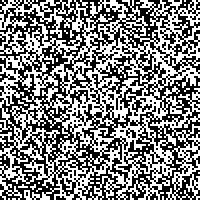
\includegraphics[width=5cm]{matrizL100Ciclo0.png}
    \caption{Representação gráfica da matriz de estados iniciais de uma simulação com $L=100$. Células pretas representam o estado $-1$ e células brancas representam o estado $+1$. A matriz de estados iniciais é gerada de forma aleatória, com semente baseada no horário de execução da simulação.}
    \label{fig:matrizL100Ciclo0}
\end{figure}

A implementação do InCA foi planejada para imprimir várias informações sobre a situação da matriz: Ciclo, Estado Médio da matriz, Limiar Médio da matriz, e Número de Aglomerados. Um \textit{Ciclo} foi definido como sendo igual a $L\times L$ atualizações aleatórias de células na matriz, já que esse seria o número de atualizações de células caso o sistema fosse determinístico. Diferentemente de \cite{stauffer}, que executou as simulações somente para vizinhanças de VonNeumann (as 4 células ortogonais à célula central, nas posições norte, sul, leste e oeste), nós também fizemos as simulações para vizinhanças de Moore, que considera as 8 células vizinhas de uma célula central.

\section{O algoritmo de contagem de aglomerados}

O grande diferencial desta implementação do InCA, em relação ao estudo de Stauffer, foi a utilização de um algoritmo de contagem de aglomerados de células com o mesmo estado. Esse algoritmo, ilustrado na Figura \ref{fig:contamination}, encontra todas as células em um mesmo aglomerado através de ``contaminações'' sucessivas de células com o mesmo estado que são vizinhas ortogonais entre si. Nós desenvolvemos este algoritmo porque o algoritmo de Hoshen-Kopelman, utilizado na pesquisa de Kramer, se mostrou muito ineficiente e demorado.

\begin{figure}
    \centering
    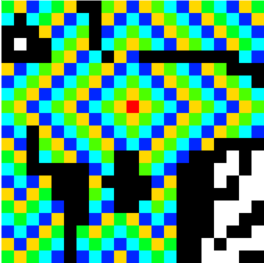
\includegraphics[width=5cm]{contamination.png}
    \caption{Algoritmo de contagem de aglomerados por contaminação de células ortogonalmente vizinhas e com o mesmo estado. Cada aglomerado é contaminado a partir de uma primeira célula até que não existam mais células a serem contaminadas. Na figura, a primeira célula é a central (em vermelho). Em seguida, as quatro células adjacentes a essa célula são contaminadas. No passo seguinte as oito células adjacentes a essas quatro células são contaminadas. O processo é repetido até que não existam mais células a serem contaminadas.}
    \label{fig:contamination}
\end{figure}

 Definiremos, matematicamente, uma \index{contaminação}\textbf{contaminação} como: dado um conjunto $C_0$ de células com o mesmo estado numa matriz ortogonal, a contaminação de $C_0$ é denotada por $\overline{C_0}$ e definida como sendo o conjunto que tem por elementos todas as células da matriz que têm alguma célula de $C_0$ ortogonalmente vizinha e estão no mesmo estado das células de $C_0$. 

 Utilizando a definição acima, definiremos o algoritmo de contagem de aglomerados de células \texttt{+1} em uma matriz finita assim: 
\begin{enumerate}
	\item crie uma matriz booleana auxiliar de mesma dimensão e tamanho que a matriz original de células e inicie ela com o valor \texttt{false};
	%\item passando por cada célula da matriz original, verifique se o valor na posição correspondente na matriz auxiliar está em \texttt{true} ou o estado da célula na matriz original é \texttt{-1}. Se qualquer uma dessas interrogações for verdadeira, passe para a próxima célula da matriz original, repetindo este passo. Caso contrário, realize o próximo passo;
	%\item marque a posição correspondente da célula na matriz auxiliar como \texttt{true} e adicione a mesma a uma fila de espera (\textit{queue}). 
	\item passe por cada célula $c_i$ da matriz original. Se o estado da célula for \texttt{-1}, pule para a próxima célula. Se a posição correspondente dessa célula na matriz auxiliar tiver valor \texttt{true}, pule para a próxima célula. Caso contrário, execute o passo abaixo.
	\item dado o conjunto unitário inicial $C_0=\{c_i\}$, itere contaminações até que $C_n=\overline{C_n}$. Marque as posições equivalentes das células em $C_n$ na matriz auxiliar como \texttt{true}. Se o número de elementos em $C_n$ for maior que $1$, incremente o contador de número de aglomerados.
	\item repita o passo 2 até que todas as células da matriz tenham sido verificadas.
\end{enumerate}

O leitor com experiência em conjuntos perceberá que o conjunto de células contaminadas no passo $n$ é dado por $\overline{C_{n-1}}-C_{n-1}=C_n-C_{n-1}$ e que quando $C_{n-1}=\overline{C_{n-1}}=C_n$ teremos que o conjunto de células contaminadas é $C_n-C_{n-1}=C_n-C_n=\emptyset$. Portanto, a condição de término do processo de contaminação é equivalente ao momento em que não existem mais células a serem contaminadas.

Este algoritmo tem complexidade $O(N)$ (vide REFERÊNCIA ALGORITHMS MANUAL), onde $N$ é o número total de células na matriz. Isso pode ser facilmente verificado, considerando que cada célula $c$ será verificada no máximo $v(c)+1$, onde $v$ é uma função que retorna o número de células de uma dada célula. Para vizinhanças de VonNeumann, esse número é $5$ e para vizinhanças de Moore esse número é $9$, ambas em duas dimensões. Esse é um avanço considerável em comparação com o algoritmo de  Hoshen-Kopelman que, por análise prória do autor deste trabalho, demonstrou ter complexidade $O(N^2)$.

\section{Metodologias de análise}

As análises foram feitas com base nos dados de estado médio, limiar médio, e número de aglomerados em função do ciclo da simulação. Nesses gráficos foram buscados padrões recorrentes, como retas, parábolas ou elipses.

\subsection{A correlação entre estado médio e número de aglomerados}

O estudo da correlação entre estado médio e número de aglomerados foi motivado pela percepção de que os gráficos de número de aglomerados \textit{versus} estado médio sempre apresentavam inclinações com o mesmo sinal. Apesar de curto, este serviu de gatilho para o estudo de afinidades.

\subsection{Afinidade}

Como mencionado acima, foi percebido que o número de aglomerados estava relacionado ao estado médio da matriz. De fato, essa relação se mostrou aproximadamente linear para todos os conjuntos de dados obtidos, como ilustrado na Figura \ref{fig:exemploAfinidade}. 
\begin{figure}[h]
    \centering
    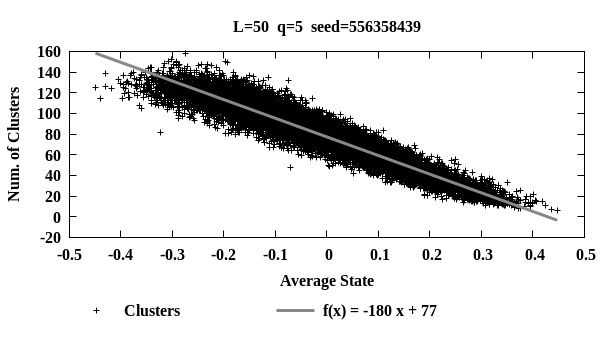
\includegraphics[width=.75\linewidth]{ICA-L50-q5_0-seed556358439-ClusterVsAvgState.png}
    \caption{Exemplo de como o número de aglomerados (eixo vertical) tende a ser linearmente dependente ao estado médio (eixo horizontal). Este gráfico contém 20000 pontos de dados obtidos numa simulação com ajuste máximo de limiar igual a $5.00$, largura de matriz igual a $50$ e vizinhança de Moore. Esse padrão foi observado em todas as outras medições realizadas. Fonte: produção própria.}
    \label{fig:exemploAfinidade}
\end{figure}
Considerando que todas as inclinações eram negativas, de modo que estados médios positivos implicavam em um número menor de aglomerados e estados médios negativos implicavam em um número maior de aglomerados, foi percebido que a inclinação da reta que melhor aproximava esses conjuntos de pontos representava a tendência de as células da matriz se aglomerarem, surgindo daí, o nome afinidade. Tecnicamente, definimos afinidade assim:

\textbf{Definição:} No InCA, seja $I_{q,L}$ a inclinação da reta que melhor aproxima os dados obtidos para número de aglomerados em função do estado médio em uma simulação com ajuste máximo de limiar igual a $q$ e largura de matriz $L$. Seja $Imin_L$ a menor inclinação encontrada entre todas as simulações para um dado $L$. Definimos a \textit{afinidade em função de $q$ e $L$} como sendo $A_{q,L}=-I_{q,L}/Imin_L$.

Esse padrão foi observado tanto para vizinhanças de VonNeumann como para vizinhanças de Moore, e os estudos foram feitos sobre como a afinidade se comporta quando os valores de $q$ e $L$ são alterados, além das diferenças entre os dados obtidos para ambas as vizinhanças.

Para a vizinhança de VonNeumann, as seguintes coleções de dados foram obtidas:\\
$\bullet$ Cinco conjunto de dados, com 20000 pontos cada, para cada combinação de $q$ e $L$ com $q\in\{$ 
  $0.1,$ $0.2,$ $0.3,$ $0.4,$ $0.5,$ $0.6,$ $0.7,$ $0.8,$ $0.9,$
  $1,$ $1.2,$ $1.4,$ $1.6,$ $1.8,$ 
  $2,$ $2.2,$ $2.4,$ $2.6,$ $2.8,$ 
  $3,$ $3.2,$ $3.4,$ $3.6,$ $3.8,$
  $4,$ $4.2,$ $4.4,$ $4.6,$ $4.8,$
  $5,$ $5.2,$ $5.4,$ $5.6,$ $5.8,$
  $6,$ $6.2,$ $6.4,$ $6.6,$ $6.8,$
  $7,$ $7.2,$ $7.4,$ $7.6,$ $7.8,$
  $8,$ $8.2,$ $8.4,$ $8.6,$ $8.8,$
  $9,$ $9.2,$ $9.4,$ $9.6,$ $9.8,$ $10,$
  $11,$ $12,$ $13,$ $14,$ $15,$ $16,$ $17,$ $18,$ $19,$ $20,$
  $22,$ $24,$ $26,$ $28,$ $30,$ $32,$ $34,$ $36,$ $38,$ $40,$
  $42,$ $44,$ $46,$ $48,$ $50,$ $52,$ $54,$ $56,$ $58,$ $60,$
  $65,$ $70,$ $75,$ $80,$ $85,$ $90,$ $95,$ $100,$ $110,$
  $120,$ $130,$ $140,$ $150,$ $160,$ $170,$ $180,$ $190,$
  $200,$ $220,$ $240,$ $260,$ $280,$ $300,$ $320,$ $340,$ $360,$ $380,$
  $400,$ $420,$ $440,$ $460,$ $480,$ $500,$ $520,$ $540,$ $560,$ $580,$
  $600,$ $620,$ $640,$ $660,$ $680,$ $700,$ $720,$ $740,$ $760,$ $780,$
  $800,$ $820,$ $840,$ $860,$ $880,$ $900,$ $920,$ $940,$ $960,$ $980,$
	$1000\}$ e $L\in \{50, 100, 250\}$.\\
	$\bullet$ Cinco conjunto de dados, com 10000 pontos cada, para $L=500$ e $q\in\{$
  $0.2,$ $0.4,$ $0.6,$ $0.8,$ $1,$
  $1.2,$ $1.4,$ $1.6,$ $1.8,$	$2,$
  $2.2,$ $2.4,$ $2.6,$ $2.8,$ $3,$
  $3.2,$ $3.4,$ $3.6,$ $3.8,$ $4,$
  $4.2,$ $4.4,$ $4.6,$ $4.8,$ $5,$
  $5.2,$ $5.4,$ $5.6,$ $5.8,$ $6,$
  $6.2,$ $6.4,$ $6.6,$ $6.8,$ $7,$
  $7.2,$ $7.4,$ $7.6,$ $7.8,$ $8,$
  $8.2,$ $8.4,$ $8.6,$ $8.8,$ $9,$
  $9.2,$ $9.4,$ $9.6,$ $9.8,$ $10$
	$\}$. \\
	Esse intervalo de $q$ entre 0 e 10 foi escolhido porque o principal fenômeno estudado acontecia entre esses valores. O tempo de simulação também foi um fator importante para a redução dos parâmetros utilizados (para $L=500$ a simulação chegou a durar mais de 12 horas, mesmo com parâmetros reduzidos).

	Já para a vizinhança de Moore, foram obtidas as seguintes coleções de dados:\\
	$\bullet$ Cinco conjuntos de 20000 pontos que considerou $L=50$ e $q\in\{$ 
  $0.1,$ $0.2,$ $0.3,$ $0.4,$ $0.5,$ $0.6,$ $0.7,$ $0.8,$ $0.9,$
  $1,$ $1.2,$ $1.4,$ $1.6,$ $1.8,$ 
  $2,$ $2.2,$ $2.4,$ $2.6,$ $2.8,$ 
  $3,$ $3.2,$ $3.4,$ $3.6,$ $3.8,$
  $4,$ $4.2,$ $4.4,$ $4.6,$ $4.8,$
  $5,$ $5.2,$ $5.4,$ $5.6,$ $5.8,$
  $6,$ $6.2,$ $6.4,$ $6.6,$ $6.8,$
  $7,$ $7.2,$ $7.4,$ $7.6,$ $7.8,$
  $8,$ $8.2,$ $8.4,$ $8.6,$ $8.8,$
  $9,$ $9.2,$ $9.4,$ $9.6,$ $9.8,$ $10,$
  $11,$ $12,$ $13,$ $14,$ $15,$ $16,$ $17,$ $18,$ $19,$ $20,$
  $22,$ $24,$ $26,$ $28,$ $30,$ $32,$ $34,$ $36,$ $38,$ $40,$
  $42,$ $44,$ $46,$ $48,$ $50,$ $52,$ $54,$ $56,$ $58,$ $60,$
  $65,$ $70,$ $75,$ $80,$ $85,$ $90,$ $95,$ $100,$ $110,$
  $120,$ $130,$ $140,$ $150,$ $160,$ $170,$ $180,$ $190,$
  $200,$ $220,$ $240,$ $260,$ $280,$ $300,$ $320,$ $340,$ $360,$ $380,$
  $400,$ $420,$ $440,$ $460,$ $480,$ $500,$ $520,$ $540,$ $560,$ $580,$
  $600,$ $620,$ $640,$ $660,$ $680,$ $700,$ $720,$ $740,$ $760,$ $780,$
  $800,$ $820,$ $840,$ $860,$ $880,$ $900,$ $920,$ $940,$ $960,$ $980,$
  $1000\}$. \\
	$\bullet$ Cinco conjuntos de 10000 pontos que considerou $L\in\{$ $100,$ $250,$ $500$ $\}$  e $q\in\{$ 
  $0.2,$ $0.4,$ $0.6,$ $0.8,$
  $1,$ $1.2,$ $1.4,$ $1.6,$ $1.8,$ 
  $2,$ $2.2,$ $2.4,$ $2.6,$ $2.8,$ 
  $3,$ $3.2,$ $3.4,$ $3.6,$ $3.8,$
  $4,$ $4.2,$ $4.4,$ $4.6,$ $4.8,$
  $5,$ $5.2,$ $5.4,$ $5.6,$ $5.8,$
  $6,$ $6.2,$ $6.4,$ $6.6,$ $6.8,$
  $7,$ $7.2,$ $7.4,$ $7.6,$ $7.8,$
  $8,$ $8.2,$ $8.4,$ $8.6,$ $8.8,$
  $9,$ $9.2,$ $9.4,$ $9.6,$ $9.8,$ $10,$
  $11,$ $12,$ $13,$ $14,$ $15,$ $16,$ $17,$ $18,$ $19,$ $20,$
  $22,$ $24,$ $26,$ $28,$ $30,$ $32,$ $34,$ $36,$ $38,$ $40,$
	$42,$ $44,$ $46,$ $48,$ $50$ $\}$\\
	$\bullet$ Obtenção de cinco conjuntos de 10000 pontos, para uma simulação que utilizou a vizinhança de Moore (8 células adjacentes), e considerou $L=500$  e $q\in\{$ 
  $0.2,$ $0.4,$ $0.6,$ $0.8,$
  $1,$ $1.2,$ $1.4,$ $1.6,$ $1.8,$ 
  $2,$ $2.2,$ $2.4,$ $2.6,$ $2.8,$ 
  $3,$ $3.2,$ $3.4,$ $3.6,$ $3.8,$
  $4,$ $4.2,$ $4.4,$ $4.6,$ $4.8,$
  $5,$ $5.2,$ $5.4,$ $5.6,$ $5.8,$
  $6,$ $6.2,$ $6.4,$ $6.6,$ $6.8,$
  $7,$ $7.2,$ $7.4,$ $7.6,$ $7.8,$
  $8,$ $8.2,$ $8.4,$ $8.6,$ $8.8,$
  $9,$ $9.2,$ $9.4,$ $9.6,$ $9.8,$ $10$ $\}$
\subsection{Caos}

Considerando que computadores geram números aleatórios a partir de uma \textit{seed}, foi verificada a presença de caos utilizando o seguinte método:
  \begin{enumerate}
    \item Geração da matriz inicial com uma \textit{seed} $S1$ (gerada com a função de números aleatórios de uma calculadora Casio);
    \item Inversão do sinal do estado e do limiar de $n$ células em posições aleatórias geradas com uma \textit{seed} baseada no horário mundial;
    \item Execução da simulação para 10000 ciclos utilizando $L=100$, limiar igual a $q$ e uma \textit{seed} igual a $S2$ (também gerada em uma Casio);
  \end{enumerate}
	Esse procedimento foi feito para $n\in\{0, 1, 10, 100, 1000, 10000\}$ e $q\in\{0.1, 1,$ $2,$ $3,$ $4,$ $5,$ $6,$ $7,$ $8,$ $9,$ $10\}$.\\
  Para a vizinhança de VonNeumann foram utilizadas as \textit{seeds} $S1=263598624$ e $S2=33386826$. Para a vizinhança de Moore foram utilizadas as \textit{seeds} $S1=156501936$ e $S2=2376222$. Representações gráficas dessas sementes estão dispostas nas Figuras \ref{fig:matrizInicialCaosMoore} e \ref{fig:matrizInicialCaosVonNeumann}.
  \begin{figure}[h]
    \subfloat[Matriz estado. Em branco o estado \texttt{-1}. Em preto o estado \texttt{+1}.]
    {
      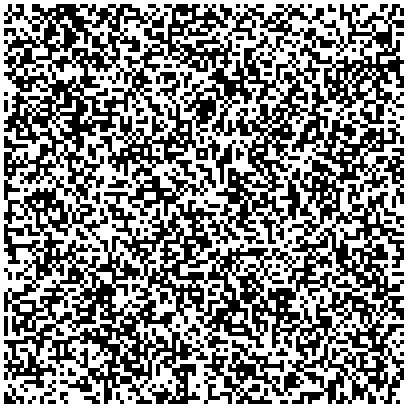
\includegraphics[width=0.45\textwidth]{seed156501936.png}
    }\hfill
    \subfloat[Matriz limiar normalizada. Em branco o limiar mais alto. Em preto o limiar mais negativo.]
    {
      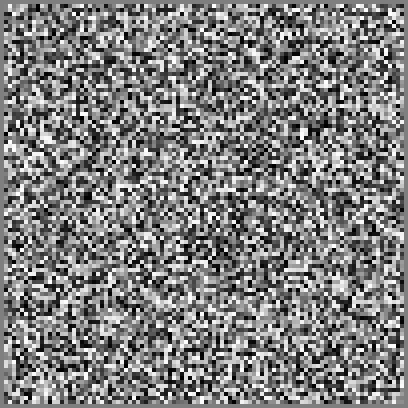
\includegraphics[width=0.45\textwidth]{seed156501936thres.png}
    }
    \caption{Matrizes iniciais geradas com a \textit{seed} 156501936. Essas matrizes foram utilizadas em todas as simulações de estudo de caos com vizinhança de Moore.}
    \label{fig:matrizInicialCaosMoore}
  \end{figure}

  \begin{figure}
    \subfloat[Matriz estado. Em branco o estado \texttt{-1}. Em preto o estado \texttt{+1}.]
    {
      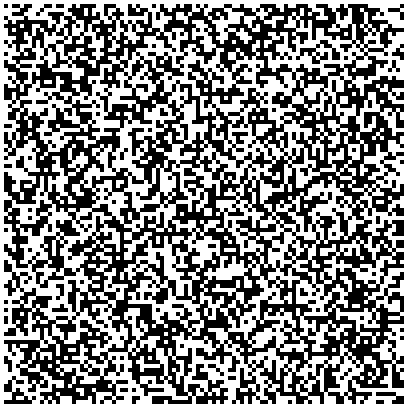
\includegraphics[width=0.45\textwidth]{seed263598624.png}
    }\hfill
    \subfloat[Matriz limiar normalizada. Em branco o limiar mais alto. Em preto o limiar mais negativo.]
    {
      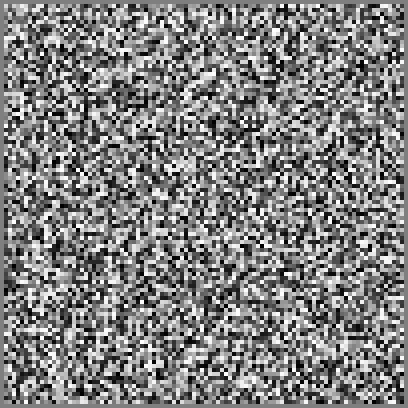
\includegraphics[width=0.45\textwidth]{seed263598624thres.png}
    }
    \caption{Matrizes iniciais geradas com a \textit{seed} 263598624. Essas matrizes foram utilizadas em todas as simulações de estudo de caos com vizinhança de VonNeumann.}
    \label{fig:matrizInicialCaosVonNeumann}
  \end{figure}
	

  A verificação da existência de caos foi feita considerando o coeficiente de Lyapunov
  \begin{align}
    \lambda = \dfrac{1}{n} \mathrm{ln}\left|\dfrac{f^n(x+\varepsilon) - f^n(x_0)}{\varepsilon}\right| = \dfrac{1}{n} \mathrm{ln}(\Delta)
  \end{align}
  Porém, considerando que $\mathrm{ln}(0)=-\infty$ e que computadores não lidam muito bem com infinito, foram feitas as seguintes observações com o intuito de desenvolver um coeficiente equivalente:
  \begin{enumerate}
    \item $\forall \Delta > 0$ tem-se que $\lambda < 0 \Leftrightarrow \mathrm{e}^\lambda < 1 \Leftrightarrow \Delta^\frac{1}{n} < 1 \Leftrightarrow \Delta^\frac{1}{10} < 1 \Rightarrow$ sistema estável 
    \item $\forall \Delta > 0$ tem-se que $\lambda = 0 \Leftrightarrow \mathrm{e}^\lambda = 1 \Leftrightarrow \Delta^\frac{1}{n} = 1 \Leftrightarrow \Delta^\frac{1}{10} = 1$ 
    \item $\forall \Delta > 0$ tem-se que $\lambda > 0 \Leftrightarrow \mathrm{e}^\lambda > 1 \Leftrightarrow \Delta^\frac{1}{n} > 1 \Leftrightarrow \Delta^\frac{1}{10} > 1 \Rightarrow$ sistema caótico 
  \end{enumerate}
 (O número 10 foi tomado arbitrariamente com a finalidade de diminuir números grandes). Portanto, para demonstrar que existe caos no sistema estudado é suficiente mostrar que $\Delta^\frac{1}{10} > 1$. 
 
 A verificação da quantidade de caos foi feita listando os valores médios de $\Delta^\frac{1}{10}$ para matrizes iniciais que tiveram entre $0.01\%$ a $100\%$ de suas células modificadas, para ambos os tipos de vizinhanças.

\chapter{Resultados e Análises}

O primeiro estudo foi realizado quanto ao efeito da topologia no comportamento do valor médio e do limiar médio em função do ciclo. Foi observado que topologias com bordas conectadas apresentam gráficos mais suaves em relação a topologias com bordas fechadas. %Isso está ilustrado nas Figuras \ref{fig:topocaixa} e \ref{fig:topotorus}.

%\begin{figure}
%    \centering
%    \includegraphics[width=.9\linewidth]{topocaixa%.png}
%    \caption{Topologia de caixa}
%    \label{fig:topocaixa}
%\end{figure}
%
%\begin{figure}
%    \centering
%    \includegraphics[width=.9\linewidth]{topotorus%.png}
%    \caption{Topologia de Torus}
%    \label{fig:topotorus}
%\end{figure}

O segundo estudo foi feito quanto ao número de aglomerados e índice de células pertencentes a aglomerados. Também foi explorada a relação entre estado médio e número de aglomerados. Foi observado que o índice de células em aglomerados aumenta quando o estado médio fica positivo, como ilustrado na Figura \ref{fig:dataL2000Q100CellInClusterAvgStateVsCycle}. 
\begin{figure}[h]
    \centering
    %\includegraphics[width=.9\linewidth]{dataL2000Q100CellInClusterAvgStateVsCycle.png}
    \caption{Demonstração da correlação entre o índice de células positivas que pertencem a algum aglomerado e o estado médio do sistema. Quando o estado médio fica mais positivo (existem mais células positivas), o índice de células positivas em aglomerados aumenta proporcionalmente. Analogamente, se o estado médio diminui, o índice de células positivas em aglomerados também diminui.}
    \label{fig:dataL2000Q100CellInClusterAvgStateVsCycle}
\end{figure}
Isso demonstra que esses dois valores estão correlacionados, implicando que as células tendem a estarem aglomeradas. 

Quanto à relação entre o número de aglomerados em função do estado médio, foi constatado que estes tendem a estar relacionados linearmente como na Figura \ref{fig:dataL1750Q100ClustersVsAvgState}. 
\begin{figure}[h]
    \centering
    %\includegraphics[width=.9\linewidth]{dataL1750Q100ClustersVsAvgState.png}
    \caption{Exemplo da tendência de o número de aglomerados tender a ser linearmente dependente ao estado médio. Este gráfico contém 300 pontos de dados obtidos numa simulação com ajuste máximo de limiar igual a $1.00$ e largura de matriz igual a $1750$. Esse padrão foi observado em todas as outras medições realizadas.}
    \label{fig:dataL1750Q100ClustersVsAvgState}
\end{figure}
Uma análise dos coeficientes angulares das retas que melhor aproximam esses dados (através do Método dos Mínimos Quadrados) para várias larguras de matrizes e vários valores de ajuste máximo de limiar revelou que os gráficos desses coeficientes angulares em função de $q$ apresentam um ``vale'' semelhante ao do potencial de Lennard-Jones, como exibido na Figura \ref{fig:DadosSlopeL1000}.
\begin{figure}
    \centering
    %\includegraphics[width=.9\linewidth]{DadosSlopeL1000.png}
    \caption{Exemplo da curva  em função do ajuste máximo de limiar $q$ encontrada para a maioria dos gráficos das inclinações do número de aglomerados \textit{versus} estado médio. Inicialmente foi conjecturada uma semelhança como potencial de Lennard-Jones.}
    \label{fig:DadosSlopeL1000}
\end{figure}
A presença desse ``poço'' em todas as simulações realizadas incentivou a definição da afinidade em função do ajuste máximo de limiar.

\textbf{Definição:} No InCA, seja $I_{q,L}$ a inclinação da reta que melhor aproxima os dados obtidos em uma simulação com ajuste máximo de limiar igual a $q$ e largura de matriz $L$. Seja $Imin_L$ a menor inclinação para um dado $L$. Definimos a \textit{afinidade em função de $q$ e $L$} como sendo $A_{q,L}=-I_{q,L}/Imin_L$.

Contudo, ao analisar a afinidade para várias larguras $L$ diferentes, foi verificado que a Afinidade independe da largura da matriz, como está exibido na Figura \ref{fig:afinidadesQ0a200L750a2000}.
\begin{figure}
    \centering
    %\includegraphics[width=.9\linewidth]{afinidadesQ0a200L750a2000.png}
    \caption{Demonstração da independência da afinidade em relação à largura $L$ da matriz utilizada nas simulações. A sobreposição das seis curvas é aproximadamente absoluta até $q\approx 30$, divergindo levemente entre $q\approx 50$ e $q\approx 200$ devido à natureza estocástica da simulação.}
    \label{fig:afinidadesQ0a200L750a2000}
\end{figure}
Esse fato, corroborado pelo mapa da Figura \ref{fig:afinidadesHeatmap},
incentiva a seguinte definição:

\textbf{Definição:} A \textit{afinidade em função de $q$} é dada pelo valor médio da \textit{afinidade em função de $q$ e $L$} através de várias medições para vários valores de $L$.

Com base nessa definição, foi encontrado o gráfico da afinidade através das simulações realizadas. Esse gráfico está exibido na Figura \ref{fig:afinidadeMedia}.

Também foram buscados padrões de caos e atratores na dinâmica não-linear das simulações realizadas, sendo encontrados vários gráficos com comportamentos interessantes, como o da Figura \ref{fig:dataL1000Q75ClustersVsAvgThres}. Contudo, ainda não foi verificado se existe caos nesses sistemas.

Por fim foram feitas simulações considerando matrizes em três dimensões, nas quais foi possível constatar comportamentos análogos aos observados no caso de duas dimensões, como a relação entre estado médio e limiar médio em função do ciclo de simulação, além da linearidade do número de aglomerados em função do estado médio. Trabalhos nessas simulações foram descontinuados devido a incertezas sobre a precisão do código utilizado.

\section{Fenômenos não estudados}

% ----------------------------------------------------------
% Finaliza a parte no bookmark do PDF
% para que se inicie o bookmark na raiz
% e adiciona espaço de parte no Sumário
% ----------------------------------------------------------
\phantompart

% ---
% Conclusão
% ---
\chapter{Conclusão}
% ---

Com os trabalhos desenvolvidos neste semestre foi possível desenvolver habilidades de análise e reprodução de autômatos celulares (em especial o \textit{Inhomogenous Cellular Automata} de Stauffer). A grande surpresa do estudo aconteceu nos recorrentes padrões lineares no caso dos gráficos do número de aglomerados em função do estado médio, sendo ainda mais surpreendente a independência da afinidade em relação à largura da matriz utilizada. A existência de discos como atratores de vários dos gráficos de número número de aglomeros em função do limiar médio também foi inesperada. Dos estudos relacionados à simulações em três dimensões, foi fortalecida a necessidade de códigos de programação bem organizados, a fim de evitar incertezas sobre a validade dos resultados.

Os próximos passos incluem estudar o motivo da existência do máximo no gráfico da afinidade média (Figura \ref{fig:afinidadeMedia}), possivelmente relacionando-o ao potencial de Lennard-Jones, analisar os atratores nos gráficos do número de aglomerados em função do limiar médio utilizando teoria de dinâmica não-linear e caos, e explorar autômatos não lineares em dimensões maiores do que 2.

% ----------------------------------------------------------
% ELEMENTOS PÓS-TEXTUAIS
% ----------------------------------------------------------
\postextual
% ----------------------------------------------------------

% ----------------------------------------------------------
% Referências bibliográficas
% ----------------------------------------------------------
\bibliography{abntex2-modelo-references}

% ----------------------------------------------------------
% Glossário
% ----------------------------------------------------------
%
% Consulte o manual da classe abntex2 para orientações sobre o glossário.
%
%\glossary

% ----------------------------------------------------------
% Apêndices
% ----------------------------------------------------------

% ---
% Inicia os apêndices
% ---
\begin{apendicesenv}

% Imprime uma página indicando o início dos apêndices
\partapendices

% ----------------------------------------------------------
\chapter{Quisque libero justo}
% ----------------------------------------------------------

\lipsum[50]

% ----------------------------------------------------------
\chapter{Nullam elementum urna vel imperdiet sodales elit ipsum pharetra ligula
ac pretium ante justo a nulla curabitur tristique arcu eu metus}
% ----------------------------------------------------------
\lipsum[55-57]

\end{apendicesenv}
% ---


% ----------------------------------------------------------
% Anexos
% ----------------------------------------------------------

% ---
% Inicia os anexos
% ---
\begin{anexosenv}

% Imprime uma página indicando o início dos anexos
\partanexos

% ---
\chapter{Morbi ultrices rutrum lorem.}
% ---
\lipsum[30]

% ---
\chapter{Cras non urna sed feugiat cum sociis natoque penatibus et magnis dis
parturient montes nascetur ridiculus mus}
% ---

\lipsum[31]

% ---
\chapter{Fusce facilisis lacinia dui}
% ---

\lipsum[32]

\end{anexosenv}

%---------------------------------------------------------------------
% INDICE REMISSIVO
%---------------------------------------------------------------------
\phantompart
\printindex
%---------------------------------------------------------------------

\end{document}
